\documentclass{book}

\usepackage[utf8]{inputenc}
\usepackage{titlesec}
\usepackage{easylist}
\usepackage{hanging}
\usepackage{hyperref}
\usepackage[a4paper,top=2.0cm,bottom=2.0cm,left=2.0cm,right=3.0cm]{geometry}
\usepackage{blindtext}
\usepackage{tipa}
\usepackage{epigraph}
\usepackage{enumerate}
\usepackage{longtable}
\usepackage{setspace}
\usepackage{verbatim}
\usepackage[T1]{fontenc}
\usepackage{graphicx}
\usepackage[italian]{babel}
\usepackage{amsmath}
\usepackage{pbox}
\usepackage{fancyhdr}
\usepackage{cancel}
\usepackage{tabularx}
\usepackage{booktabs}
\usepackage{multirow}
\usepackage{longtable}
\usepackage{upgreek}
\usepackage{tikz}
\usepackage{tikz-qtree}
\usepackage{subfig}
\usepackage{xcolor}
\usepackage{amssymb}
\usepackage{mathrsfs}
\usepackage{textcomp}
\usepackage{circuitikz}
\usepackage{pifont}
\usepackage{mathtools}
\usepackage{amsmath}
\usepackage{listings}
\usepackage{color}
\usepackage{tasks}
\usepackage{amsthm}
%\usepackage{epstopdf} %converting to PDF

\newtheorem{defi}{Definizione}
\newtheorem{nota}{Nota}
\newtheorem{esempio}{Esempio}
\newtheorem{teo}{Teorema}
\usetikzlibrary{angles, arrows.meta, quotes}
\usepackage{siunitx}

\definecolor{mygreen}{rgb}{0,0.6,0}
\definecolor{mygray}{rgb}{0.5,0.5,0.5}
\definecolor{mymauve}{rgb}{0.58,0,0.82}

\lstset{ 
  backgroundcolor=\color{white},   % choose the background color; you must add \usepackage{color} or \usepackage{xcolor}; should come as last argument
  basicstyle=\footnotesize,        % the size of the fonts that are used for the code
  breakatwhitespace=false,         % sets if automatic breaks should only happen at whitespace
  breaklines=true,                 % sets automatic line breaking
  captionpos=b,                    % sets the caption-position to bottom
  commentstyle=\color{mygreen},    % comment style
  deletekeywords={...},            % if you want to delete keywords from the given language
  escapeinside={\%*}{*)},          % if you want to add LaTeX within your code
  extendedchars=true,              % lets you use non-ASCII characters; for 8-bits encodings only, does not work with UTF-8
  firstnumber=1000,                % start line enumeration with line 1000
  frame=single,	                   % adds a frame around the code
  keepspaces=true,                 % keeps spaces in text, useful for keeping indentation of code (possibly needs columns=flexible)
  keywordstyle=\color{blue},       % keyword style
  language=Octave,                 % the language of the code
  morekeywords={*,...},            % if you want to add more keywords to the set
  numbers=left,                    % where to put the line-numbers; possible values are (none, left, right)
  numbersep=5pt,                   % how far the line-numbers are from the code
  numberstyle=\tiny\color{mygray}, % the style that is used for the line-numbers
  rulecolor=\color{black},         % if not set, the frame-color may be changed on line-breaks within not-black text (e.g. comments (green here))
  showspaces=false,                % show spaces everywhere adding particular underscores; it overrides 'showstringspaces'
  showstringspaces=false,          % underline spaces within strings only
  showtabs=false,                  % show tabs within strings adding particular underscores
  stepnumber=2,                    % the step between two line-numbers. If it's 1, each line will be numbered
  stringstyle=\color{mymauve},     % string literal style
  tabsize=2,	                   % sets default tabsize to 2 spaces
  title=\lstname                   % show the filename of files included with \lstinputlisting; also try caption instead of title
}

\linespread{1.5} % l'interlinea

\frenchspacing

\newcommand{\abs}[1]{\lvert#1\rvert}

\usepackage{floatflt,epsfig}

\usepackage{multicol}
\newcommand\yellowbigsqcup[1][\displaystyle]{%
  \fboxrule0pt
  \ifx#1\textstyle\fboxsep-0.6pt\else\fboxsep-1.25pt\fi
  \mathrel{\fcolorbox{white}{yellow}{$#1\bigsqcup$}}}

\title{Appunti Fisica}
\author{Nicola Ferru}
\date{}

\begin{document}
\maketitle
\tableofcontents
\listoftables
\listoffigures
% pagine dedicate
\section{Premesse\dots}

In questo repository, inoltre,  sono disponibili le dimostrazioni grafiche realizzate
con \textit{Geogebra}; consiglio a tutte le persone che usufruiranno di questo lavoro, di dare un occhiata alle dimostrazioni grafiche e stare attenti,  in quanto nel tempo potranno  essere presenti delle modifiche, cosi da apportare miglioramenti al contenuto degli stessi appunti.  Solitamente il lavoro di revisione viene fatto tre/quattro volte alla settimana perché sono in piena fase di sviluppo.  Ricordo a tutti che essendo un progetto volontario ci potrebbero essere dei rallentamenti per cause di ordine superiore e quindi
potrebbero esserci meno modifiche del solito oppure essere presenti degli errori.  Chiedo pertanto  la cortesia a voi lettori di contattarmi per apportare eventuali correzioni .  Tengo a precisare che tutto il progetto è puramente open source, pertanto vengono resi disponibili i sorgenti dei file LaTex  insieme ai PDF compilati.

\begin{center}
	Cordiali saluti
\end{center}
\newpage

\section{Simboli}
\begin{multicols}{3}
	$\in$ Appartiene\\
	$\notin$ Non appartiene\\
	$\exists$ Esiste\\
	$\exists !$ Esiste unico\\
	$\subset$ Contenuto strettamente\\
	$\subseteq$ Contenuto\\
	$\supset$ Contenuto strettamente\\
	$\supseteq$ Contiene\\
	$\Rightarrow$ Implica\\
	$\Longleftrightarrow$ Se e solo se\\
	$\neq$ Diverso\\
	$\forall$ Per ogni\\
	$\ni :$ Tale che\\
	$\leq$ Minore o uguale\\
	$\geq$ Maggiore o uguale\\
	$\alpha$ alfa\\
	$\beta$ beta\\
	$\gamma$ gamma\\
	$\Gamma$ Gamma\\
	$\delta,\Delta$ delta\\
	$\epsilon$ epsilon\\
	$\sigma,\Sigma$ sigma\\
	$\rho$ rho
\end{multicols}

\part{fisica 1}
\input{pag/unita di misura.tex}
\chapter{L'Energia}
\section{Lavoro}
\begin{defi}
	Il lavoro è definito come il prodotto della forza per lo spostamento del
	suo punto di applicazione. Esso è quindi uno scalare
	\begin{equation}
		L=\vec{F}*\vec{s}=Fs\cos \theta
	\end{equation}
	In cui $\theta$ è l'angolo più piccolo formato tra la forza e lo
	spostamento
	\begin{equation*}
		\begin{matrix}
			\text{Dimensioni: } & [L]=[F][L]=[MLT^{-2}][l]=[ML^2T^{-2}]\\
			\text{Unita in misura: } & Kg m^2 s^{-2} = \text{Joule simbolo (J)}
		\end{matrix}
	\end{equation*}
	$L=\vec{F}*\vec{s}=Fs\cos\theta$
	\begin{equation*}
		\begin{matrix}
			L>0 &\Rightarrow \cos \theta>0 &\Rightarrow \theta < \frac{\pi}{2}=90^o\\
			L=0 &\Rightarrow \cos \theta=0 &\Rightarrow \theta =
			\frac{\pi}{2}\\
			L<0& \Rightarrow \cos \theta <0 & \Rightarrow \theta > \frac{\pi}{2}
		\end{matrix}
	\end{equation*}
\end{defi}
\subsection{Lavoro di più forza costanti sullo stesso corpo}
Il lavoro totale è la somma di tutti i lavori fatti dalle forza (costanti) che
agiscono sul sistema considerato.
\begin{equation*}
	\begin{matrix}
	L_T=\vec{F}_1+\vec{s} +
	\dots+\vec{F}_n*\vec{s}=\displaystyle\sum_{i=1}^{n}
	\vec{F}_i*\vec{s}=\left(\displaystyle\sum_{i=1}^{n}
	\vec{F}_i\right)*\vec{R}*\vec{s} &
		\vec{R}=\left(\displaystyle\sum_{i=1}^{n}\right) \vec{F}_i
	\end{matrix}
\end{equation*}
$\vec{R}$ = Risultante delle Forze
\begin{esempio}
	Calcolare il lavoro fatto dalla forza agenti su una cassa di massa m=50.0Kg
	trascinata, per una distanza di 6,00 metri su un piano liscio, mediamente
	una corda con tensione T pari a 200N che forma un angolo di 35,0° con
	l'asse delle x.
	\begin{equation*}
		L_T=L_{\vec{N}}+L_{\vec{T}_y} + L_{\vec{T}_x} L_{\vec{p}}
	\end{equation*}
	\begin{equation*}
		\begin{cases}
			\vec{N}\\
			\vec{T}_y\\
			\vec{P}
		\end{cases}
		\text{sono tutte perpendicolare allo spostamento } \vec{s} \Rightarrow
		L_N + L_{\vec{T}_y} + L_{\vec{p}} = 0
	\end{equation*}
	\begin{equation*}
		L_T=L_{\vec{T}_x}=\vec{T}_x*\vec{s}=Ts\cos \theta = 200N*6m*0,82 \cong
		\boxed{983 joule}
	\end{equation*}
\end{esempio}
\begin{esempio}
	Calcolare il lavoro fatto dalle forze agenti su una cassa massa $m=50Kg$
	trascinata, per una distanza di 6 metri su un piano scabro (attrito
	$\mu=0,15$), mediante una corda con tensione T pari a 200N che forma un
	angolo di 35° con l'asse delle x.
        \begin{center}
            \fbox
            {
            \begin{minipage}{0.75\textwidth}
                    Forza d'attrito
                    \begin{equation*}
                            f_d=\mu_d N^\prime=\mu_d(mg-T_y) \Rightarrow f_d=\mu_d[mg-T\sin
                            35^o]=56,4 Newton
                    \end{equation*}
            \end{minipage}
            }
      	\end{center}
	\paragraph{Lavoro Totale}
	\begin{equation*}
		L_T=L_{\vec{N}}+L_{\vec{T}_y} + L_{\vec{T}_x}+L_{\vec{p}} +
		L_{\vec{f}_d}
	\end{equation*}
	\begin{equation*}
		\begin{cases}
			\vec{N}\\
			\vec{T}_y\\
			\vec{P}
		\end{cases}
		\text{sono tutte perpendicolare allo spostamento } \vec{s} \Rightarrow
		L_N + L_{\vec{T}_y} + L_{\vec{p}} = 0
	\end{equation*}
	\begin{equation*}
		L_T=L_{\vec{T}_x} + L_{\vec{f}_d}=\vec{T}_x*\vec{s} + \vec{f}_d
		*\vec{s} =[T\cos \theta s \cos 0^o +f_ds\cos \pi]
	\end{equation*}
	\begin{equation*}
		L_T=\{(200*0,82*6*1)+[56,4*6*(-1)]\} Joule \cong \boxed{646J}
	\end{equation*}
\end{esempio}
\subsection{Lavoro di una forza variabile unidimensionale}
\begin{defi}
  La forza varia della posizione\footnote{Come ad esempio in una molla stirata in una direzione}.
  Ogni volta che pasiamo da una posizione $x_i$ a quella $x_j$ la forza varia e compie il lavoro.
  Se $x_i$ è molto prossimo a $x_j$ la forza varierà poco e quindi possiamo definire il lavoro
  elementare come:
  \begin{equation*}
    dL=\vec{F}*\Delta\vec{x}=F\Delta x \text{ La forza è compresa tra i valori che
      essa assume in $x_i$ e $x_j$.}
  \end{equation*}
  Il lavoro si ottiene sommando i lavori infinitesimi fatti dalla forza durante lo spostamento del
  suo punto di applicazione $x_1$ e $x_2$ e quindi coincide con l'area L.
  \begin{equation*}
    L_T=\sum_{i=1}^N dL=F_idx \text{ Se $\Delta x \to 0$, invece } L_T=\int_{x_1}^{x_2} F_x dx
  \end{equation*}
  Il lavoro di una forza rappresenta quindi l'area\footnote{attenzione L ha le dimensioni di una
    forza per una lunghezza} della regione al disotto della curva che pappresenta la variazione
  della forza in funzione dello spostamento, regione celeste nella figura sotto.
  \clearpage
  \begin{figure}[th]
    \centering
    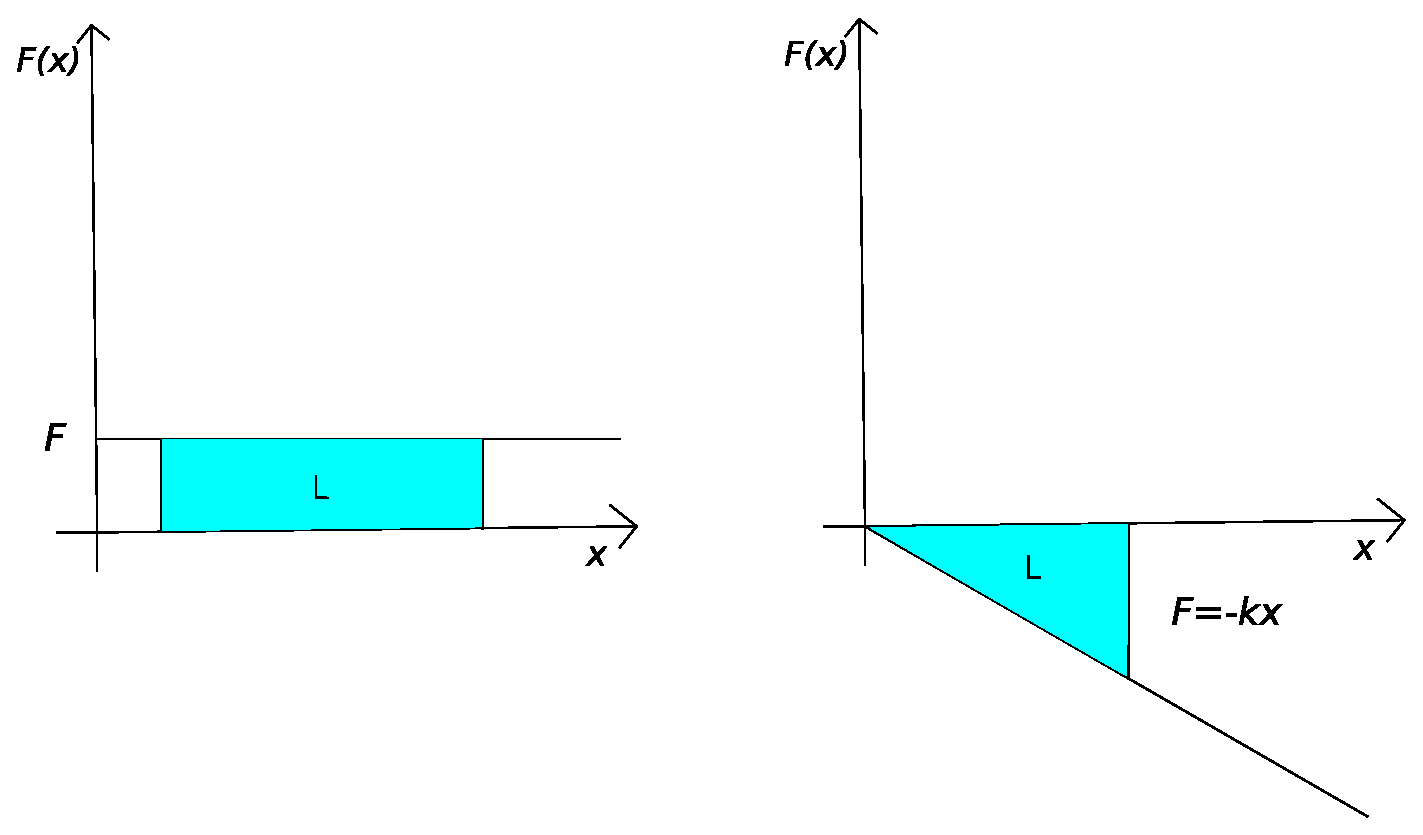
\includegraphics[width=8cm]{img/finiti/forze_costanti_e_elastiche.eps}
    \caption{Forze costanti e elastiche}
  \end{figure}
\end{defi}
\begin{nota}
  Nel caso della figura a sinistra si tratta di una forza costante, mentre, quella di destra è una
  forza elastica, come si vede nel caso della prima si presenta come un rettangolo che per
  l'appunto mantiene un intensità costante, mentre nel caso del secondo, ha un andamento che segue
  la funzione $F= -kx$
\end{nota}
\subsubsection{Lavoro della forza variabile prodotta dalle molle (Forza elastica)}
\begin{figure}[th]
    \centering
    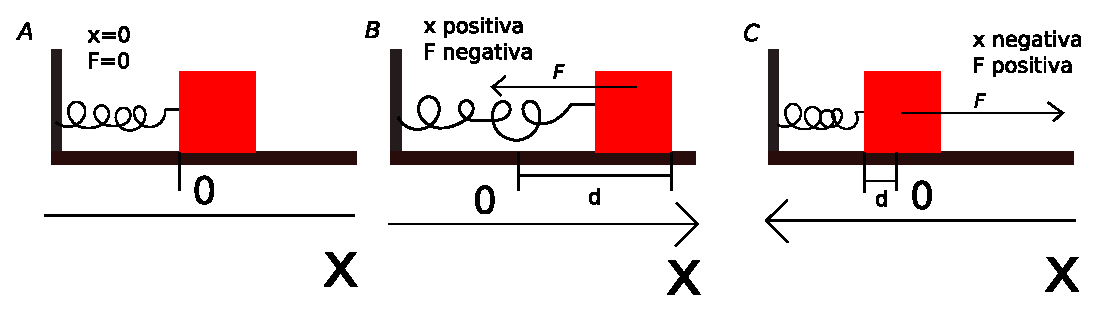
\includegraphics[width=10cm]{img/finiti/forza_elastica.eps}
    \caption{Forza elastica}
\end{figure}
\begin{equation}
  L_T=\int^{x}_0 \vec{F}_x*d\vec{x}=\int^x_0(-kx)dx=-1/2kx^2
\end{equation}

\begin{esempio}
  Calcolare il lavoro fatto dalla forza elastica di una molla avente $k=450\frac{N}{m}$ quando
  essa è stirata di 15 cm rispetto alla  sua posizione di riposo.
  \begin{equation}
    L_{F_e}= -1/2 kx^2=-0,5 * 450 \frac{N}{m}*(0,15m)^2=-5,06Nm=-5,06J
  \end{equation}
\end{esempio}
\clearpage
\subsection{Teorema dell’Energia Cinetica (caso unidimensionale forza costante)}
Consideriamo una forza $\vec{F}$ costante che agisce un corpo di massa m che sposta il suo punto di
applicazione di una quantità $\vec{s}$
\begin{figure}[th]
    \centering
    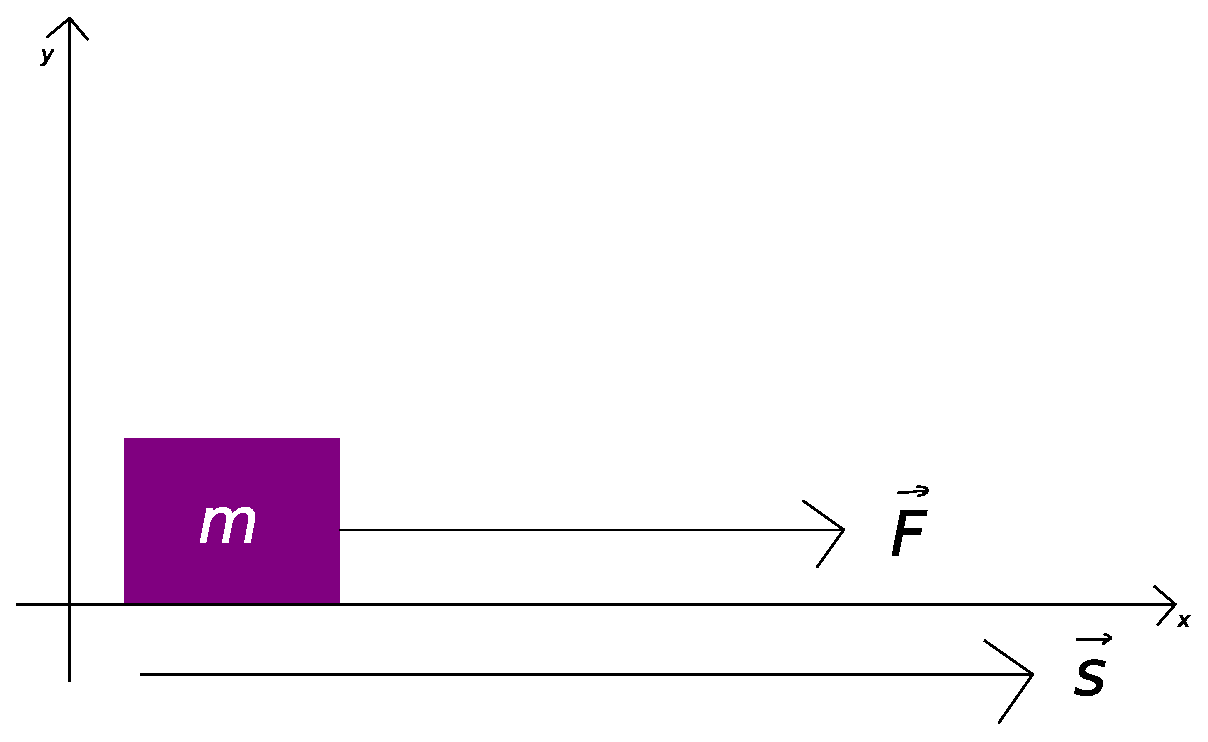
\includegraphics[width=10cm]{img/finiti/forza_costante.eps}
    \caption{Forza costante}
\end{figure}
\begin{equation}
  \begin{matrix}
    F=ma & a=\frac{F}{m}=costante \Rightarrow \text{ Moto naturalmente accelerato}
  \end{matrix}
\end{equation}
Abbiamo quindi che $v_2^2+2a(x_2-x_1)$ \footnote{Dove ($x_2-x_1$) è il modulo dello spostamento}
\begin{equation}
  L=\vec{F} * Fs \cos 0 = ma (x_2-x_1)=m\frac{v_2^2-v_1^2}{2(x_2-x_1)}(x_2-x_1)
\end{equation}
\begin{teo}
  In fisica, il teorema dell'energia cinetica (o teorema lavoro-energia, o
  teorema delle forze vive) afferma che se un corpo possiede un'energia cinetica iniziale e
  una forza agisce su di esso effettuando un lavoro, l'energia cinetica finale del corpo è
  uguale alla somma dell'energia cinetica iniziale e del lavoro compiuto dalla forza lungo
  la traiettoria del moto.
  \begin{equation}
    L=\frac{1}{2} m v_2^2-\frac{1}{2} m v_1^2=K_2-K_1=K_f-K_i=\Delta K
  \end{equation}
\end{teo}
\subsection{Lavoro di una forza variabile in 3 dimensioni}
\begin{figure}[th]
    \centering
    \includegraphics[width=6cm]{img/finiti/forza_vet_3d.eps}
    \caption{Forza vettoriale in 3 dimensioni}
\end{figure}
\begin{eqnarray*}
	\vec{S}=\displaystyle\sum_{i=1}^{N}\vec{S}_i & \begin{matrix}
		\text{Spostamento totale}\\
		\text{come limite della spezzata per}\\
		N\to \infty
	\end{matrix}\\
	& \vec{F}=F_x\vec{i}+\vec{F}_y\vec{j}+\vec{F}_z\vec{k}\\
	& d\vec{s}=dx\vec{i}+dy\vec{j}+dz\vec{k}
\end{eqnarray*}
Quindi si può dire che $L_T=\displaystyle\sum_{i=1}^{N}\vec{F}_i*\vec{s}_i\to
L_T=\int_{A}^{B}\vec{F}*d\vec{S}$, se e solo se $\abs{\vec{s}_i}\to 0$
\subsubsection{Teorema dell'energia cinematica tridimensionali}
\begin{eqnarray*}
	\vec{F}=F_x\vec{i}+\vec{F}_y\vec{j}+\vec{F}_z\vec{k}
	& d\vec{s}=dx\vec{i}+dy\vec{j}+dz\vec{k}
\end{eqnarray*}
\begin{eqnarray*}
	L=\int \vec{F}*d\vec{s}=\int
	\left(F_xd_x+F_yd_y+F_zdz\right)=\int_{x_1}^{x_2}ma_xdx+\int_{y_1}^{y_2}
	ma_ydy+\int_{x_1}^{z_2}ma_zdz\\ = \int_{x_1}^{x_2}m\frac{dv_x}{dt}dx+
	\int_{y_1}^{y_2}m\frac{dv_y}{dt}dy+\int_{z_1}^{z_2}m\frac{dy_z}{dt}dz=
	\int_{v_{x_1}}^{v_{x_2}}mv_xdv_x+\int_{v_{y_1}}^{v_{y_2}} mv_ydv_y
	+\int_{v_{x_1}}^{v_{z_2}}mv_zdv_z\\
	=\frac{1}{2}m\left[v_x^2\right]_{v_{x_1}}^{v_{x_2}}+ 
	\frac{1}{2}m\left[v_y^2\right]_{v_{y_1}}^{v_{y_2}}+\frac{1}{2}m
	\left[v_z^2\right]_{v_{z_1}}^{v_{z_2}}=
	\frac{1}{2}m\left[v_{x_2}^2-v_{x_1}^2\right]+
	\frac{1}{2}m\left[v_{y_2}^2-v_{y_1}^2\right]+
	\frac{1}{2}m\left[v_{z_2}^2-v_{z_1}^2\right]\\
	=\frac{1}{2}m\left[v_{x_2}^2+v_{y_2}^2+v_{z_2}^2\right]
	-\frac{1}{2}m\left[v_{x_1}^2+v_{y_1}^2+v_{z_1}^2\right]=\frac{1}{2}mv_2^2
	-\frac{1}{2}mv_1^2
\end{eqnarray*}
Quindi alla fine il risultato è 
\begin{equation*}
	\boxed{L=\frac{1}{2}mv_2^2
	-\frac{1}{2}mv_1^2}
\end{equation*}
Il lavoro fatto dalla forza ({\it risultante}) applicata al sistema è quindi
legato alla variazione della velocità del sistema durante l’applicazione della
forza stessa.
\section{Teorema dell'energia cinetica}
\begin{defi}
	L'energia cinetica è l'energia che possiede un corpo per il movimento che ha
	o che acquista: equivale al lavoro necessario per portare un corpo da una 
	velocità nulla a una velocità nota. Quando un corpo di massa m varia la sua 
	velocità, con questa varia anche la sua energia cinetica. Il lavoro equivale
	a questa variazione di energia cinetica. L'energia cinetica quindi è
	associata alla massa e alla velocità di un corpo in movimento. L'energia
	cinetica che possiede un corpo di massa m nel suo moto di caduta è uguale al
	lavoro compiuto per fermarsi.
\end{defi}
Matematicamente, l'energia cinetica è $K=\frac{1}{2}mv^2$ -- Il lavoro totale
fatto dalle forza che agiscono sul sistema considerato, è uguale alla
variazione della sua energia cinematica:
\begin{equation*}
	\boxed{L_T=L=\frac{1}{2}mv_2^2-\frac{1}{2}mv_1^2=K_2-K_1=K_f-K_i=\Delta K}
\end{equation*}
L'energia cinetica è uno scalare che ha le stesse dimensioni del Lavoro. Si
misura quindi in Joule ({\tt J})
\begin{equation*}
	[K]=[ML^2T^{-2}] \text{ Unità di misura: Joule (J)}
\end{equation*}
Lavoro ed Energia cinetica
\begin{eqnarray*}
	L_T>0\Rightarrow \Delta K>0 &v_f>v_i & \text{Il sistema accelera}\\
	L_T=0\Rightarrow \Delta K=0 &v_f=v_i & \text{La velocità del sistema rimane
	invariata}\\
	L_T<0\Rightarrow \Delta K<0 &v_f<v_i & \text{Il sistema decelera}
\end{eqnarray*}
\chapter{Modelli atomici}
\section{Modello atomico di Bohr-Sommerfeld}
Il modello atomico proposto da Niels Bohr nel 1913, successivamente ampliato da Arnold Sommerfeld nel 1916, è la più famosa applicazione della quantizzazione dell'energia che, insieme alle spiegazioni teoriche sulla radiazione del corpo nero, sull'effetto fotoelettrico e sullo scattering Compton, e all'equazione di Schrödinger, costituiscono la base della meccanica quantistica.\\
Il modello, proposto inizialmente per l'atomo di idrogeno, riusciva anche a spiegare, entro il margine di errore statistico, l'esistenza dello spettro sperimentale. Bohr presenta così un modello dell'atomo, facendo intuire che gli elettroni si muovono su degli orbitali. \textit{Questo modello viene ancora utilizzato nello studio dei Semiconduttori.} 
\begin{center}
	By \href{https://it.wikipedia.org/wiki/Modello_atomico_di_Bohr}{Wikipedia}
\end{center}
\part {Fisica 2}
\chapter{programma}
\section{Base}
\begin{itemize}
	\item \textit{Elettrostatica nel vuoto} - carica elettrica, legge di Coulomb, campo elettrico, teorema di Gauss e $1^a$ equazione di Maxwell, potenziale elettrico, dipolo elettrico, conduttori, capacità elettrica, sistemi di condensatori, collegamento in serie e in parallelo, energia del campo elettrostatico.
	\item \textit{Corrente elettrica stazionaria} - resistenza elettrica e legge di Ohm, effetto Joule, forza elettromotrice e generatori elettrici, circuiti in corrente continua.
	\item \textit{Magnetismo nel vuoto} - forza di Lorentz, vettore induzione magnetica, forze magnetica
	 su una corrente, momento magnetico della spira percorsa da corrente, relazione tra momento
	 meccanico e momento magnetico, campi generati da correnti stazionarie, legge di Biot e Savart (campo
	 del filo indefinito, della spira circolare e del solenoide), 2a equazione di Maxwell, teorema di Ampère.
	\item \textit{Campi magnetici variabili nel tempo} - induzione elettromagnetica , legge di 
	Faraday-Newmann, $3^a$ e $4^a$ equazione di Maxwell, autoinduzione, circuito RL, 
	energia magnetica.
	\item \textit{Onde} - equazione d'onda, tipi di onde, velocità di fase, equazioni delle onde
	elettromagnetiche e loro proprietà, onda piana e onde sferiche, energia di un'onda 
	elettromagnetica e vettore di Poynting, spettro della radiazione elettromagnetica. 
\end{itemize}
\section{Argomenti aggiuntivi}
\begin{itemize}
	\item \textit{Elettrostatica nella materia} - la costante dielettrica, interpretazione microscopica, suscettibilità elettrica.
	\item \textit{Magnetismo nella materia} - vettori B, H e M, materiali paramagnetici, ferromagnetici, diamagnetici, legge di Curie, ciclo di isteresi.
\end{itemize}

\chapter{La legge di Couloumb}
\section{Introduzione}
L'elettromagnetismo costituisce il fondamento su cui sono costruiti i computer,
le radio e televisori, le telecomunicazioni, illuminazioni ecc.
L'elettromagnetismo spiega come gli atomi siano tenuti insieme, come
avvengono i fulmini, le aurore e gli arcobaleni. Gli antichi filosofi greci
scoprirono che l'ambra strofinata attrae pagliuzze sottili e che pietre
magnetiche naturali attraggono pezzetti di ferro. Tra i tanti scienziati che
svilupparono l'elettromagnetismo moderno, notiamo il fisico sperimentale
\texttt{Michael Faraday} ed il teorico \texttt{James Clerk Maxwell}.
\subsection{La carica elettrica}
Una bacchetta di vetro strofinata con seta si \texttt{allontana} da un'altra
bacchetta di vetro strofinata con della seta.
\begin{enumerate}
	\item \textit{Forza repulsiva} - Una bacchetta di vetro strofinata con
		della seta si \textit{avvicina} ad una bacchetta di plastica strofinata
		con la pelle di camoscio.
	\item \textit{Forza attrattiva} - Le forze sono dovute alla \textbf{carica
		elettrica}.
\end{enumerate}
Esistono due tipi di carica:
\begin{enumerate}
	\item Carica positiva, contrassegnata con il segno +;
	\item Carica negativa, contrassegnata con il segno -
\end{enumerate}
Si definisce neutro un oggetto che ha le cariche positive e negative
perfettamente bilanciate.
Spostando la carica da un oggetto all'altro, si crea una carica in eccesso.
L'oggetto può scaricarsi con scintille oppure con l'umidità dell'aria.
\subsubsection{Le proprietà delle cariche}
\begin{enumerate}
	\item Le particelle cariche dello \textit{stesso segno} si respingono;
	\item Le particelle di carica opposta si attraggono;
	\item Se strofiniamo il vetro con un panno di seta risulta in una
		\textit{carica potenziale} nel vetro;
	\item Strofinando della plastica con della pelle di camoscio si ottiene una
		\textit{carica negativa} sulla stessa.
\end{enumerate}
\subsubsection{Conduttori e isolanti}
In natura esistono le seguenti tipologie di materiali:
\begin{tasks}{2}
	\task I conduttori - le cariche si muovono liberamente;
	\task Gli isolanti - le cariche non si muovono, per l'appunto restano
	isolate;
	\task I semiconduttori - le cariche si muovono, ma il materiale possiede un
	alta resistenza;
	\task I superconduttori - le cariche si muovono senza incontrare ostacoli
	di sorta.
\end{tasks}
\newtheorem{pcariche}{Particelle Cariche}
\begin{pcariche}
	La materia composte di atomi. Gli atomi hanno un \textbf{nucleo} con
	\begin{itemize}
		\item Protoni - cariche positive;
		\item Elettroni - carica negativa.
	\end{itemize}
	La carica dell'elettrone e del protone hanno la stessa intensità ma segno
	opposto. Gli elettroni sono \textbf{attratti verso il nucleo}. Nei
	conduttori, alcuni elettroni sono \textit{liberi di muoversi}, un isolante
	\textit{non ha elettroni liberi}.
\end{pcariche}
\subsection{Carica indotta}
Una carica negativa \textit{respinge} gli elettroni nel rame, risulta una
carica positiva indotta vicino alla carica esterna. Risulta una \textbf{forza
attrattiva} tra una carica negativa e un conduttore, Anche per una carica
positiva ed un conduttore la forza risulta \textbf{attrattiva}.
\section{Legge di Coulomb}
Tra due cariche puntiformi esiste una \textit{forza elettrostatica}. La forza è
diretta \textit{lungo la retta congiungente} le due cariche.
Se le cariche sono della stessa polarità le stesse si respingono, invece, se
sono di carica opposta, avviene un attrazione tra le cariche.
\subsubsection{Riassunto sui vettori}
\paragraph{Componenti:}
\begin{equation}
	F_x=F\cos 0;\text{ }F_y=F\sin 0
\end{equation}
\paragraph{Modulo e angolo:}
\begin{equation}
	F=\abs{\vec{F}}=\sqrt{F_x^2+F_y^2};\text{ } \tan 0 =\frac{F_y}{F_x}
\end{equation}
\paragraph{Versore:}
\begin{equation}
	\hat{a}=\frac{\vec{a}}{\abs{\vec{a}}}=\frac{\vec{a}}{a}
\end{equation}
\paragraph{Sommare:}
\begin{equation}
	\vec{F}=\vec{F}_1+\vec{F}_2\to F_x=F_{1x}+F_{2x};\text{ } F_y=F_{1y}+F_{2y}
\end{equation}
La forza di una carica $q_1$ in presenza di un'altra $q_2$ è:
\begin{equation}
	\vec{F}_{12}=k\frac{q_1q_2}{r^2}\hat{r}
\end{equation}
Dove $k=8,99*10^9Nm^2C^{-2}$ è la \textbf{costante di Coulomb} e $\vec{r}$ è il
vettore di lunghezza pare alla distanzia $q_2$ a $q_1$.
\begin{enumerate}
	\item Se $q_1$ e $q_2$ hanno la stessa polarità, il prodotto $q_1q_2$ è 
		\textbf{positivo} e la forza è \textit{repulsiva}.
	\item Se $q_1$ e $q_2$ hanno la polarità \textbf{opposta}, il
		prodotto $q_1q_2$ è \textbf{negativo} e la forza è \textit{attrattiva}.
\end{enumerate}
La forma è una coppia di azione-reazione: $\vec{F}_{21}=-\vec{F}_{12}$
\subsection{Unità do misura}
L'unità di carica nel SI è il \texttt{Coulomb} (\ref{}). La derivata del unità
fondamentale di corrente elettrica, \textbf{Ampere}. La corrente \textit{i} è
data dal rapporto $\frac{dq}{dt}$ con cui transita la carica \textit{q}: 
$i=\frac{dq}{dt}$.
Risulta $1C=1As$
\subsection{La costante dielettrica del vuoto}
La costante di \textit{Coulomb} viene anche espressa come
$k=\frac{1}{4\pi\xi_0}$ dove $\xi_0 = 8,85*10^{-12}C^2N^{-1}m^{-2}$ è la
\textbf{constante dielettrica del vuoto}.\\
Così scriviamo $\vec{F}=\frac{q_1q_2}{4\pi\xi_0r^2}\hat{r}$, o per ottenere il
modulo $F=\frac{\abs{q_1}\abs{q_2}}{4\pi\xi_0r^2}\hat{r}$
\subsection{Forze multiple}
Le forze elettrostatiche obbediscono al \textbf{principio di sovrapposizione}.
Se molte particelle sono vicine alla carica $q_1$, la forza netta è $\vec{F}_{1,net}=\vec{F}_{12}+\vec{F}_{14}+\dots+\vec{F}_{1n}$.
\paragraph{Attenzione:} \textit{somma vettoriale!}
\section{Teorema del guscio}
\begin{tasks}(2)
  \task Primo teorema del guscio:\\
  \textit{Una superficie sferica uniformemente carica attrae o respinge una carica esterna come se tutta la carico fasse concentroto
    nel suo centro}.
  \task Secondo teorema del guscio:\\
  \textit{Uno carico posto all'interno di uno superficie chiusa uniformemente carica non ne sente la foza}.
\end{tasks}
\section{La quantizzazione della carica}
Qualunque carica \textit{q} può essere scritta come $q=ne$ in cui $n=\pm 1,\pm 2, \pm 3, \dots$ ed è la carica elementare: $e = 1,602*10^{-19}C$
\begin{tasks}
  \task Il \textbf{protone} ha carica $+e$
  \task L'ettrone ha carica $-e$
\end{tasks}

Il valore di e è così piccolo che normalmente la granularità non appare nei fenomeni di larga scala. Attraverso un filo con corrente di 1A passano circa $6,2*10^{18}$ elettroni al secondo.

\section{La conservazione della carica}
La carica elettrica è conservata - Lo strofinamento del vetro con un panno di seta non crea carica positiva, ma trasferisce elettroni dal vetro alla seta. Anche nei processi nucleari la carica totale rimane invariata.
\section{Verifica}
\begin{enumerate}
\item Indicare il verso della forza che agisce sul protone centrale
\item Ordinare i tre casi secondo i valori decrescenti del modulo della forza netta sull'elettrone.
\end{enumerate}
\paragraph{Soluzione primo problema}
\begin{equation}
  q_1=+e,q_2=+2e, \text{ } R=2cm.
\end{equation}
Calcolo la forza $\vec{F}_{12}$
\begin{equation}
  F_{12}=k\frac{\abs{q_1}\abs{q_2}}{R^2}=k\frac{2e^2}{R^2}=\frac{8,99*10^9*2*(1,6*10^{19})}{R^2}=1,15*10^{-24}N
\end{equation}
Quindi il valore finale è $\vec{F}_{12}=-(1,15*10^{-24}N)\hat{x}$
\begin{equation}
  q_1=+e, q_2 = +2e,q_3=-2e, R=2cm.
\end{equation}
Calcolo la forza $\vec{F}_{1,net}$
\begin{equation}
 F_{13}=k\frac{2e^2}{\left(\frac{3}{4}R\right)^2}=2,05*10^{-24}N
\end{equation}
Quindi il valore che otteniamo è $F_{13}=(2,05*10^{-24}N)$
\begin{equation}
  \begin{matrix}
  \vec{F}_{1,net}=\vec{F}_{12}+\vec{F}_{13}=-(1,15*10^{-24}N)\hat{x}+(2,05*10^{-24}N)
    \hat{x}\\=(0,90*10^{24}N)\hat{y}=-(0,125*10^{-24}N)\hat{x}+(1,775*10^{-24}N)\hat{y}
  \end{matrix}
\end{equation}
Quindi il valore che otteniamo è $F_{1,net,x}=\sqrt{F^2_{1,net,x}+F^2_{1,net,y}}=1,78*10^{-24}N$
\paragraph{Soluzione secondo problema}
$q_1=8e,\text{ } q_2=-2e$. In che punto un protone è in equilibrio?
\begin{equation}
  \begin{matrix}
    \vec{F}_1+\vec{F}_2=0. \text{ } x>L.\text{ } \frac{kq_1e}{x^2}+\frac{kq_2e}{(x-L)^2}=0\\
    \to \left(\frac{x-L}{x}\right)=\frac{-q_2}{q_1}=\frac{1}{4}\to \frac{x-L}{x}=\frac{1}{2}\to x=2L
  \end{matrix}
\end{equation}


\input{pag/campi_elettrici.tex}
\chapter{La legge di Gauss}
\section{L'aspetto fisico}
Per calcolare il campo elettrico $\vec{E}$ di una distribuzione di carica si può \textbf{sommare} (integrare). La procedura è \textit{laboriosa}. Se esiste la simmetria, possiamo utilizzare un metodo più semplòice che sfrutta la relazione tra carica e campo, la \textbf{legge di Gauss}
\section{La superficie Gaussiana}
Scegliamo una superficie Gaussiana ({\it cioè una superficie chiusa}) intorno ad una carica.
Per la carica puntiforme, la {\bf sfera} è la superficie più simmetrica.
Le linee di campo intercettano la superficie.
\begin{tasks}
  \task Per una carica $Q$ il campo è $E=\frac{kQ}{r^2}$
  \task Per una carica 2Q, più linee intercettano la superficie
  \task la carica è $-\frac{Q}{2}$
\end{tasks}
Serve una grandezza che \textbf{quantifica} quanto una superificie è attraversata da un campo.
\section {Il flusso elettrico}
Un campo $\vec{E}$ attraversa un elemento di superficie $\Delta \vec{A}$ \texttt{vettore di area $\Delta \vec{A}$: \textbf{perpendicolare} alla superficie}.\\ Definizione del flusso elettrico $\Delta \vec{\upphi}$:
\begin{equation}
	\Delta \upphi =\vec{E}*\Delta\vec{A}=E\Delta A\cos\texttheta
\end{equation}
Per l'\textit{intera} superficie:
$\upphi = \sigma \vec{E}*\Delta \vec{A}=\int \vec{E}*d\vec{A}$ - Per una superficie chiusa, l'orientamento di $\Delta \vec{A}$ è uscente.
\begin{itemize}
\item $\vec{E}$ uscente contribuisce $\Delta \upphi >0$
\item $\vec{E}$ entrante contribuisce $\Delta \upphi <0$
\item $\vec{E} || \Delta \vec{A}$ da $\Delta \upphi =0$
\end{itemize}
Il flusso netto di una superficie chiusa è
\begin{equation}
	\upphi=\oint \vec{E}*d\vec{A}
\end{equation}
\section{Cilindro in campo uniforme}
Superficie guessiana a forma di \textbf{cilindro} di raggio \textit{R}. Campo elettrico $\vec{E}$
\textbf{uniforme}, parallelo all'asse. Quanto vale il fluso netto?
\begin{equation}
  \upphi=\oint \vec{E}*d\vec{A}=\int_a \vec{E}*d\vec{A}+\int_b\vec{E}*d\vec{A}+\int_c \vec{E}*
  d\vec{A}
\end{equation}
\begin{itemize}
\item $\int_a \vec{E}*d\vec{A}=-\pi R^2E$
\item $\int_b \vec{E}*d\vec{A}=0$
\item $\int_c\vec{E}*d\vec{A}=\pi R^2E$
\item $\upphi =0$  
\end{itemize}
\section{La legge di Gauss}
Relazione tra il flusso $\upphi$ attraverso una superficie chiusa e la carica netta $q_{int}$ racchiusa all'interno della superficie:
\begin{equation}
	\xi_0\upphi=q_{int} \text{ o } \xi_0\oint \vec{E}*d\vec{A}=q_{int}
\end{equation}
\begin{itemize}
\item \textit{se $q_{int}$ è positiva, il flusso netto è uscente}
\item \textit{se $q_{int}$ è negativo, il flusso netto è entrante}
\end{itemize}
Una carica esterna alla superficie può cambiare $\vec{E}$ localmente, ma non influisce sul flusso totale.
\begin{figure}[!h]
 	\centering
	\includegraphics[height=5cm]{img/cariche opposte.jpg}
    	\caption{Due cariche di intensità uguale, ma di segno opposto}
\end{figure}
\begin{itemize}
\item $S_1$: $\vec{E}$ uscente in tutti i punti. $\Phi$ positivo, $q_{int}$ negativa
\item $S_2$: $\vec{E}$ entrante in tutti i punti. $\Phi$ negativa, $q_{int}$ negativa
\item $S_3$ Non racchiude nessuna carica. Ogni linea di campo che entra, esce, quindi $\Phi = 0$
  \item $S_4$ $q_{int}$ = $Q-Q=0$, quindi $\Phi = 0$
\end{itemize}

\section{La legge di Gauss e di Coulomb}
Racchiudiamo una \textbf{carica puntiforme} in una superficie sferica di raggio $r$.
Per simmetria, il campo elettronico ha il medesimo modulo $E$ su \textbf{tutti i punti della sfera}.\\
Applichiamo Gauss:
\begin{eqnarray*}
  \xi_0\oint \vec{E}*d\vec{A}=q_{int}\\
  \xi_0 E(4\pi r^2) = q\\
  E=\frac{q}{4\pi\xi_0r^2}
\end{eqnarray*}
Cioè, la legge di coulomb!
\subsection{Problema svolto}
Guscio sferica di raggio $R=10cm$ - dotato di carica uniforme $Q=-16e$ - Al centro carca puntiforme $q=5e$. Calcolare il campo $\vec{E}$
\begin{itemize}
\item nel punto $P_1$ a $r_1=6cm$
\item nel punto $P_2$ a $r_2=12cm$
\end{itemize}
\begin{eqnarray*}
  \xi_0 E_1(4\pi r_1^2)=q\to E=\frac{q}{4\pi \xi_0 r^2_1}=\frac{4e}{4\pi \xi_0 (0,06m)^2}=2,0*10^{-6}\frac{N}{C} \text{ verso l'esterno}\\
  \xi_0 E_2 (4\pi r^2_2)=q+Q\to \frac{q+Q}{4\pi \xi_0 r^2_2}=\frac{4e}{4\pi \xi_0 (0,12m)^2}=1,1 *10^{-6}\frac{N}{C} \text{ verso l'interno}
\end{eqnarray*}
\section{Un conduttore carico isolato}
Il campo elettrico all'\textit{interno} di un conduttore in equilibrio elettrostatico è \textit{nullo}
\begin{center}
	se no, si spostano le cariche
\end{center}
Scegliamo una superficie gaussiana appena sotto la superficie. $E=0\to \phi=0\to q_{int}=0$\\
L'eccesso di carica su un conduttore isolato si dispone totalmente sulla
\textbf{superficie esterna}. Anche una superficie gaussiana che racchiude \textbf{una cavita} ha
$E=0 \to \phi=0\to q_{int}=0$. La superficie di una cavità interna di un conduttore \textbf{non ha carica} in eccesso.\\
In generale, la carica \textit{non} si distribuisce uniformemente sulla superficie di un conduttore. Però c'è una relazione diretta tra il \textbf{campo} \textit{E} e la \textbf{densità di carica} $\sigma$. Considera un ciindro che racchiude un elemento di superficie - Il campo $E$ è
\textbf {perpendicolare} alla superficie
\begin{center}
	{\it se no si sposta la carica}
\end{center}
applicando Gauss: $\xi_0 \oint \vec{E}*d\vec{A}=q_{int}\to \xi_0EA=\sigma A \to E=\frac{\sigma}{\xi_0}$
\subsection{Problema svolto}
Una carica puntiforme di $Q=-5\mu C$ è posta all'interno di un guscio sferico metallico di raggio interno $R$, spostato di una distanza $\frac{R}{2}$ dal centro.
\begin{itemize}
\item Qual'è la carica indotta?
\item Qual'è l'andamento del campo interno ed esterno?
\end{itemize}
$Q$ induce un carica positiva $+5\mu C$ di all'interno, distribuita in modo \textbf{non-uniforme}.
Il campo all'interno è asimmetrico. La parete interna ha una carica di $-5\mu C$ distribuita in modo \textbf{uniforme}. Il campo esterno è simmetrico, come il campo di una carica puntiforme.
\section{Gauss per simmetria cilidrica}
Una bacchetta di plastica, di lunghezza infinita, densità di carica pari a $\lambda C/m$, Com'è il campo $\vec{E}$ a distanza $r$? Fruttare l'integrale è davvero faticoso\dots Applichiamo Gausss per la \textbf{superficie cilintrica} di altezza $h$. Per simmetria, $\vec{E}$ ha direzione \textbf{radiale}.
\begin{equation}
\xi_9\oint \vec{E}*d\vec{A}=q_{int}\to \xi_0 E2\pi hr=\lambda h\to E=\frac{\lambda}{2\pi r\xi_0}
\end{equation}
vake se la distanza dell'estremità è molto minore di $r$.
\section{Gauss per simmetria piana}
Una lamina isolante sottile, con una densità di carica superficiale $\sigma \frac{C}{m^2}$.
\paragraph{Superficie gaussiana:} cilindro di base $A$. Per simmetria, $\vec{E}$ perpendicolare alla lamina.\\ Applichiamo Guass: $\xi \oint \vec{E}*d\vec{A}=q_{int} \to \xi_0E2A=\sigma A\to E=\frac{\sigma}{2\xi_0}$\\
Concorda con il risultato trovato per il disco $E=\frac{\sigma}{2\xi_0}\left(1-\frac{z}{\sqrt{(R^2+z^2)}}\right)$\\
Per una piastra conduttrice la carica si distribuisce sulla superficie. Senza campo esterno, la carica è uguale da ambi lati, $\sigma_1=\sigma/2$. Identico, ma con verso di $E$ opposto, per carica negativa. Messe una a cando all'altra, le cariche sono attratte verso l'intrno. Il campo in mezzo diventa $E=\frac{2\sigma_1}{\xi_0}=\frac{\sigma}{\xi_0}$
\section{Gauss per simmetria sferica}
Con Gauss dimostriamo i 2 teoremi dei gusci. Guscio sferico di carica totale $q$ e raggio $R$.
\begin{enumerate}
\item \textit{Una superficie unifomemente carica attrae o respinge una carica esterna come se tutta la carica fosse concentrata nel suo centro.} Applicare Gauss alla superficie $S_2: E=\frac{q}{4\pi \xi_0 r^2}$ per $(r>R)$
  \item \textit{Una carica posta all'interno di una superficie chiusa uniformemente carica non ne sente la forza.} Applicare Gauss alla superficie $S_2: E=q_{int}=0$ per $(r<R)$
\end{enumerate}
Ogni distribuzione con simmetira sfrefica è una sovrapposizione di strati concentrici. Densità di carica $p$ varia soltanto con $r$
\begin{equation}
  E=\frac{q^\prime}{4\pi\xi_0r^2}
\end{equation}
Per $p$ uniforme e $r<R$
\begin{equation}
  	\frac{q^\prime}{\frac{4}{3}\pi r^3}=\frac{q}{\frac{4}{3}\pi R^3}\to q^\prime=q\frac{r^3}{R^3}
\end{equation}
per ci $E=\frac{qr}{4\pi \xi_0 R^3}$

\chapter{Potenziale elettrico}
\section{L'aspetto fisico}
La forza elettrostatica è \textbf{conservativa}, per cui, si può associarvi un'\textbf{energia potenziale}. La \textbf{conservazione} dell'energia meccanica semplifica molti calcoli. $q_2$ senta la \textbf{forza} $\vec{F}$ di $q_1$. Alla posizione di $q_2$ c'è un \textbf{campo} $\vec{E}=\vec{F}/q_2$ - $q_2$ ha un \textbf{energia potenziale} \textit{U} dovuta a $q_1$. Alla posizione di $q_2$ c'è un \textbf{potenziale elettrico} $V=\frac{U}{q_2}$ (\textbf{Nota bene:} grandezza scalare!)
\section{Il potenziale elettrico}
L'energia potenziale \textit{U}: $U=0$ a un \textbf{livello di riferimento}. Spostando, la forza conservativa compie un \textbf{lavoro} $L$. L'energia potenziale è $E=-L$. Scegliamo $U=0$ a \textbf{carica esplorativa} $q_0$ viene trasportata da $\infty$ a $P$.\\
$L_\infty$ è il lavoro svolto \textbf{dalla forza elettrica} per il trasporto. Il potenziale elettrico nel punto $P$: $V=\frac{-L_\infty}{q_0}$. Ad ogni posizione interno ad una carica è assegnato un potenziale elettrico.
\section{Unità di misura}
Il potenziale elettrico viene espresso in $\frac{J}{C}$ o V (\textbf{Volt}).\\
Figura anche in altre unità:
\begin{center}
  Il campo elettrico $1\frac{N}{C}=1\frac{V}{m}$
\end{center}
L'energia per il \textbf{sistema microscopici}: $1eV=1,6*10^{-19}$
\begin{center}
  \textit{\color{blue} $1eV$ è la differenza in energia di un elettrone che attraverso una differenza di potenziale di 1V}
\end{center}
\section{Il potenziale elettrico}
\paragraph{Inversamente:} una carica $q$ in un potenziale elettrico $V$ ha energia potenziale $U=qV$. Spostanedosi in un compo elettrico da $i$ e $f$ abbiamo differenza di potenziale $\Delta V=V_f-V_i$. Per una carica $q: \Delta U=q\Delta V=q(V_f-V_i)=-L$, $\Delta V \text{ } \Delta U$ \textbf{non dipendono dal cammino} da $i$ a $f$.\\
Possibile applicare la \textbf{conservazione dell'energia meccanica: } $U_i+K_i=U_f+K_f$ per cui $\Delta K=K_f-K_i=-q\Delta V$ - Se agisce sulla particella anche un'altra forza che compie un lavoro $L_{app}$, abbiamo $\Delta K=-q\Delta V+L_{L_{app}}$.
\section{Superfici equipotenziali}
L'insieme dei punti con lo \textbf{stezzo potenziale} forma una superficie: La superficie equipotenziale. Spostando una carica tra due punti di una superficie equipotenziale, il campo elettrico \textbf{non compie lavoro}.\\
Spostamenti \textbf{sulla} superficie hanno $L=0$, per cui $L=\vec{F}*\vec{d}=q \text{ } \vec{E}*\vec{d}=qEd\cos\theta=0\to \theta =90^o$\\
La superficie equipotenziale è perpendicolare a $\vec{E}$
\begin{itemize}
\item \textit{Per un campo uniforme: piani perpendicolari a $\vec{E}$}
\item \textit{Per un carica puntiforme: sfere concentriche}
\end{itemize}
\section {Calcolo del potenziale, dato $\vec{E}$}
La Carica di prova $q_0$ si muove da $i$ e $f$. Lavoro svolto da $\vec{E}$ per spostamento $d\vec{s}$:
\begin{equation}
	dL=\vec{F}*d\vec{s}=q_0\vec{E}*d\vec{s}
\end{equation}
Per cui $V_f-V_i=-\frac{L}{q_0}=-\int^f_i \vec{E}*d\vec{s}$
\begin{center}
	Non dipende dal percorso?
\end{center}
Per campo uniforme:
\begin{equation}
  \Delta V=-\int_i^f \vec{E}*d\vec{s}=-E\Delta x
\end{equation}
\section{Potenziale di una carica puntiforma}
Potenziale $V$ per punto $P$ a distanza $R$ da carica $q$. $V=0$ a distanza infinita. $V_f-V_i=-\int^f_i\vec{E}*d\vec{s}$.\\
Libertà di scelta per il cammino. Lungo la direzione radiale: $\vec{E}*d\vec{s}=Edr0-V=-\int^\infty_REdr=-\int^\infty_R\frac{q}{4\pi \xi_0r}dr=-\frac{q}{4\pi \xi_0}\left[\frac{-1}{r}\right]^\infty_R=-\frac{q}{4\pi \xi_0 r}$\\
per cui $V=\frac{q}{4\pi\xi_or}$
\begin{itemize}
\item Carica positiva $\leftrightarrow$ potenziale positivo
\item Carica negativa $\leftrightarrow$ potenziale negativo
\end{itemize}
Valido anceh per distribuzione sferiche non-puntiforme
\section{Insieme di cariche puntiformi}
Il \textit{principio di sovrapposizione} vale anche per $V$, Per $n$ cariche, il potenziale netto sarà
\begin{equation}
  V=\sum_{i=1}^{n}V_i=\frac{1}{4\pi \xi_0}\sum_{i=1}^{n}\frac{q_i}{r_i}
\end{equation}
$Nb$: somma scalare!
\subsection{problema}
due protoni. Ordinare secondo i valori crescenti di $V$ nel punto $P$
\begin{equation}
  \begin{matrix}
    q_1=+12nC\\
    q_2=-24nC\\
    q_3=+31nC\\
    q_4=+17nC\\
    d=1,3m
  \end{matrix}
\end{equation}
Qual'è il potenziale nel punto P?
\begin{equation}
  V=\frac{1}{4\pi \xi_0}\sum_{i=1}^{n}\frac{q_i}{r_i}=
  \frac{1}{4\pi\xi_0}\left(\frac{q_1}{r_1}+\frac{q_2}{r_2}+\frac{q_3}{r_3}
    +\frac{q_4}{r_4}\right)=\frac{1}{4\pi\xi_0}
  \frac{(12-24+31+17)*10^{-9}}{\frac{1,3}{\sqrt{2}}}=352V
\end{equation}
\section{Potenziale di un dipolo elettrico}
Il potenziale in un in un punto arbitrario $P$ a distanza $r$, angolo $\Theta$:
\begin{equation}
  V=V_++V_- =\frac{1}{4\pi\xi_0}\left(\frac{q}{r_+} - \frac{q}{r_-}\right)=
  \frac{q}{4\pi\xi_0}\frac{r_--r_+}{r_+r_-}
\end{equation}
Per $r>>d:r_--r_+\approx d \cos\Theta,\text{ } r_+r_-\approx r^2$
\begin{equation*}
  \to V = \frac{q}{4\pi\xi_0}\frac{d\cos \Theta}{r^2}=\frac{p\cos\Theta}{4\pi\xi_0}=
  \frac{\overrightarrow{p}*\hat{r}}{4\pi\xi_0}
\end{equation*}
Ove $\overrightarrow{r}$ è il momento dipolare -- \textit{\color{blue}il verso va da -q a +q}
\section{Potenziale di una distribuzione contitua}
Per distribuzione continua dividiamo in infinitesimi $dq$. Ogni infinitesimo $dq$ contribuisce $dV=\frac{dq}{4\pi\xi_0r}$, così $v=\frac{1}{4\pi\xi_0}\sum^n\limits_{i=0}\frac{q_i}{r_i}$ diventa $V=\frac{1}{4\pi\xi_0}\int \frac{dq}{r}$
\end{document}
